% !TeX spellcheck = en_US
\documentclass[11pt, a4paper]{article}

% Set the title of the current document to be produced.
\newcommand{\doctitle}{The comprehensive Bathymetric Lidar Uncertainty Estimator (cBLUE)}
% Command for the due date of the homework.
\newcommand{\duedate}{}

%------------------------------------------------------------
% Import commands for both teacher and course information.  | 
% NOTE: Change your teacher and course info in these files. |
%------>------>------>------>------>------>------>------>-->|
%-------------------------------------------------
% Teacher-specific commands                      |
%---------------                                 |
%-> Instructions: change your teacher info here. |
%------->------>------>------>------>------>---->|
%
\newcommand{\instructor}{Forrest Corcoran}
\newcommand{\college}{Oregon State University}
\newcommand{\email}{corcoraf@oregonstate.edu}
                              %|
%-------------------------------------------------
% Course-specific commands                       |
%---------------                                 |
%-> Instructions: change your course info here.  |
%------->------>------>------>------>------>---->|
%
\newcommand{\semester}{\ }
\newcommand{\csection}{\ }
\newcommand{\ponderation}{\ }
\newcommand{\coursetitle}{CBlue}
\newcommand{\coursenumber}{[V3.0.0]}
\newcommand{\prerequisite}{}
                               %|   
%
%------------------------------------------------------------
%-- Import packages and custom command definitons.          |
%------>------>------>------>------>------>------>------>-->|
%----------------------------------------------------
% The following is a list of LaTeX packages imports |
%------->------>------>------>------>------>---->---|
%

% The margins at the bottom of the page has been reduced.
% this allows for a slim footer.
\usepackage[left=1in,right=1in,top=1in,bottom=0.7in]{geometry}
% Original size:
%\usepackage[inner=1.5cm,outer=1.5cm,top=1.5cm,bottom=.5cm,margin=1in]{geometry}
\usepackage[
    colorlinks,
    pagebackref,
    pdfusetitle,
    urlcolor=blue,
    citecolor=blue,
    linkcolor=blue,    
    plainpages=false]
{hyperref}            
% ftp://ftp.dante.de/tex-archive/fonts/bbding/bbding.pdf
%https://ctan.math.illinois.edu/fonts/bbding/bbding.pdf
\usepackage{fancyhdr, lastpage, bbding, pmboxdraw}
\usepackage{fancyvrb}
\PassOptionsToPackage{usenames,dvipsnames}{xcolor}
\usepackage{acronym}
\usepackage{amsthm}
\usepackage{caption}
\usepackage{xcolor}
\usepackage{enumitem}
\usepackage{tabularx}
\usepackage{sectsty}
\sectionfont{\LARGE\raggedright}
\subsectionfont{\Large\raggedright}
\subsubsectionfont{\large\raggedright}
% pifont package doc at: https://ctan.math.ca/tex-archive/macros/latex/required/psnfss/psnfss2e.pdf
% pifont is used to define custom list and style list items using the \ding command. 
\usepackage{pifont} 
% bclogo used for making a colored box for notes. 
% @see: https://ctan.org/pkg/bclogo?lang=en
\usepackage[tikz]{bclogo} 
\usepackage{titlesec}  
\usepackage[open,openlevel=1]{bookmark}

%-- @see http://ctan.sharelatex.com/tex-archive/fonts/fontawesome/doc/fontawesome.pdf
% Font Awesome  http://ctan.math.washington.edu/tex-archive/fonts/fontawesome5/doc/fontawesome5.pdf
% https://muug.ca/mirror/ctan/fonts/fontawesome5/doc/fontawesome5.pdf
%\usepackage{fontawesome5}
\usepackage{fontawesome}
%---------------------------------
% ==== Font setup.
% Load any of the following fonts.
%---------------------------------
%\usepackage{lmodern}
%\usepackage{mathptmx}
%\usepackage{times}
%\usepackage[sc]{mathpazo} % Palatino font.
%\linespread{1.05} % Palatino needs more leading (space between lines)
\usepackage{tgbonum} % For Bonum/Bookman font.
\usepackage[utf8]{inputenc}
\usepackage[T1]{fontenc}
%---------------------------------
\usepackage{booktabs} 

\pagestyle{empty}
\usepackage{graphicx}
\usepackage[export]{adjustbox}
\usepackage{multicol}
\usepackage{blindtext}  
\usepackage{vhistory} % for making a table for the revision history.
\usepackage{float}
\usepackage{amsmath}
\usepackage{subfig}

%dummy text - delete me later - no problem!
\usepackage{lipsum}
                                  %|  
%--------------------------------------------------------
%--> \customhrule: makes a customized rule whose width  | 
%                  should be passed as parameter.       |
%--------------------------------------------------------
\newcommand{\customhrule}[1]{
	\rule[1.4pt]{\linewidth}{#1}
}
%------------------------------------------------------
%--> \doublerule: makes a double rule.                |
%------------------------------------------------------ 
\newcommand{\doublerule}[1][.4pt]{
	\noindent
	\makebox[0pt][l]{\rule[.7ex]{\linewidth}{#1}}%
	\rule[1pt]{\linewidth}{#1}\par} 
%===== Custom Ruler commands  ==================
\renewcommand{\headrulewidth}{1pt}
\renewcommand{\footrulewidth}{0.4pt}

% Disable spaces between list items in a labeled list.
\setlist{noitemsep}
 
%-------------------------------------------------------------
%= The followig are declaraions of custom Lists              =
%-------------------------------------------------------------
%
%======= Green rectangles list =======================
% \Rectangle from bbind
\newlist{greenrectangles}{itemize}{4}
%\setlist[greenrectangles]{topsep=4pt,partopsep=0pt,itemsep=3pt,parsep=0pt,labelindent=0.5cm,leftmargin=*}
\setlist[greenrectangles]{itemsep=5pt,parsep=0pt,topsep=4pt,partopsep=3pt}
\setlist[greenrectangles,1]{font=\color{darkred},label={\color{darkgreen}{\Rectangle}}}

%======= Alphabetical  list =======================
\newlist{alphalist}{enumerate}{9}
\setlist[alphalist]{topsep=4pt,partopsep=0pt,itemsep=3pt,parsep=0pt,labelindent=0.5cm,leftmargin=*}
\setlist[alphalist,1]{label=\textbf{\alph*)}}
%======= Non-numbered list =======================
\newlist{itemizedlist}{itemize}{9}
\setlist[itemizedlist]{topsep=4pt,partopsep=0pt,itemsep=3pt,parsep=0pt,labelindent=0.5cm,leftmargin=*}
%\setlist[itemizedlist,1 ]{label=\textbf{\alph*)}}

%======= Arrowed list =======================
\newlist{arrows}{itemize}{4}
\setlist[arrows]{topsep=4pt,partopsep=0pt,itemsep=3pt,parsep=0pt,labelindent=0.5cm,leftmargin=*}
\setlist[arrows,1]{font=\color{darkred},label={\HandRight}}

%======= Bordered square list =======================
% Colorize the selected symbol? 
% ❏
\newlist{borderedsquare}{itemize}{4}
\setlist[borderedsquare]{topsep=4pt,partopsep=0pt,itemsep=3pt,parsep=0pt,labelindent=0.5cm,leftmargin=*}
\setlist[borderedsquare,1]{label=\ding{111}}

%======= Filled, curved arrow list =======================
\newlist{curveddarrow}{itemize}{4}
\setlist[curveddarrow]{topsep=4pt,partopsep=0pt,itemsep=3pt,parsep=0pt,labelindent=0.5cm,leftmargin=*}
\setlist[curveddarrow,1]{label=\small\faMarker}

%======= Colored pen list ======================= 
\newlist{coloredPen}{itemize}{4}
\setlist[coloredPen]{topsep=4pt,partopsep=0pt,itemsep=3pt,parsep=0pt,labelindent=0.5cm,leftmargin=*}
\setlist[coloredPen,1]{font=\color{darkred},label=\small\faMarker}

%======= Objectives list ======================= 
% ➠
\newlist{objectives}{itemize}{4}
\setlist[objectives]{topsep=4pt,partopsep=0pt,itemsep=3pt,parsep=0pt,labelindent=0.5cm,leftmargin=*}
\setlist[objectives,1]{label=\small\ding{224}}

%======= Dark starred list ======================= 
% ✸
\newlist{filledstarlist}{itemize}{4}
\setlist[filledstarlist]{topsep=4pt,partopsep=0pt,itemsep=3pt,parsep=0pt,labelindent=0.5cm,leftmargin=*}
\setlist[filledstarlist,1]{label=\small\ding{88}}

%======= Dark-bordered empty circle list ======================= 
% ❍
\newlist{emptyCircleList}{itemize}{4}
\setlist[emptyCircleList]{topsep=4pt,partopsep=0pt,itemsep=3pt,parsep=0pt,labelindent=0.5cm,leftmargin=*}
\setlist[emptyCircleList,1]{label=\small\ding{109}}

%======= Filled right arrow list ======================= 
% ➤
\newlist{filledRightArrowList}{itemize}{4}
\setlist[filledRightArrowList]{topsep=4pt,partopsep=0pt,itemsep=3pt,parsep=0pt,labelindent=0.5cm,leftmargin=*}
\setlist[filledRightArrowList,1]{label=\small\ding{228}}

%======= Numbered list: non-filled circle list ======================= 
% ➀
\newlist{numberedEmptyList}{itemize}{9}
\setlist[numberedEmptyList]{topsep=4pt,partopsep=0pt,itemsep=3pt,parsep=0pt,labelindent=0.5cm,leftmargin=*}
\setlist[numberedEmptyList,9]{label=\ding{182}}

%======= Right hand pointing list =======================
\newlist{rightHandPointingList}{itemize}{4}
\setlist[rightHandPointingList]{topsep=4pt,partopsep=0pt,itemsep=3pt,parsep=0pt,labelindent=0.5cm,leftmargin=*}
\setlist[rightHandPointingList,1]{font=\color{darkred},label={\HandRight}}

%----------------------------------------------------------------------
%=   The followig are custom colors declaraions                       |
%--  more colors codes can be found at: http://latexcolor.com/        | 
%-- usage: {\color{declared-color} some text}.                        |    
%  e.g.,: {\color{darkblue}{ This text will appear darkblue-colored}} |
%----------------------------------------------------------------------
\definecolor{darkblue}{rgb}{0,0,.6}
\definecolor{darkred}{rgb}{.7,0,0}
\definecolor{darkgreen}{rgb}{0,.6,0}
\definecolor{darkestred}{rgb}{.8,.1,0}
\definecolor{red}{rgb}{.98,0,0}
\definecolor{OliveGreen}{cmyk}{0.64,0,0.95,0.40}
\definecolor{CadetBlue}{cmyk}{0.62,0.57,0.23,0}
\definecolor{lightlightgray}{gray}{0.93}
\definecolor{vanierred}{RGB}{210,0,2}
\definecolor{darkestblue}{rgb}{0.0, 0.0, 0.55}
\definecolor{darkblue}{rgb}{0,0,.6}
\definecolor{darkred}{rgb}{.7,0,0}
\definecolor{darkgreen}{rgb}{0,.6,0}
\definecolor{darkestred}{rgb}{.8,.1,0}
\definecolor{red}{rgb}{.98,0,0}
\definecolor{OliveGreen}{cmyk}{0.64,0,0.95,0.40}
\definecolor{CadetBlue}{cmyk}{0.62,0.57,0.23,0}
\definecolor{lightlightgray}{gray}{0.93}
\definecolor{darkorange}{rgb}{255,140,0}
\definecolor{fluorescentyellow}{rgb}{0.8, 1.0, 0.0}
\definecolor{darkyellow}{rgb}{1,1,0.34}
\definecolor{lightyellow}{rgb}{1,1,0.6}
\definecolor{coolblack}{rgb}{0.0, 0.18, 0.39}
\definecolor{lightgray}{rgb}{.9,.9,.9}
\definecolor{darkgray}{rgb}{.4,.4,.4}
\definecolor{purple}{rgb}{0.65, 0.12, 0.82}
\definecolor{gray}{rgb}{0.4,0.4,0.4}
\definecolor{cyan}{rgb}{0.0,0.6,0.6}
\definecolor{dkgreen}{rgb}{0,0.6,0}
\definecolor{gray}{rgb}{0.5,0.5,0.5}
\definecolor{mauve}{rgb}{0.58,0,0.82}
\definecolor{lightblue}{rgb}{0.0,0.0,0.9}
\colorlet{punct}{red!60!black}
\definecolor{background}{HTML}{EEEEEE}
\definecolor{delim}{RGB}{20,105,176}
\colorlet{numb}{magenta!60!black}
\definecolor{coolblack}{rgb}{0.0, 0.18, 0.39}
\definecolor{forestgreen}{rgb}{0.0, 0.27, 0.13}
\definecolor{firebrick}{rgb}{0.7, 0.13, 0.13}
\definecolor{rltred}{rgb}{0.75,0,0}
\definecolor{rltgreen}{rgb}{0,0.5,0}
\definecolor{rltblue}{rgb}{0,0,0.75}
\definecolor{indigo}{rgb}{0.0, 0.25, 0.42}
\definecolor{jazzberryjam}{rgb}{0.65, 0.04, 0.37}
\definecolor{lava}{rgb}{0.81, 0.06, 0.13}
\definecolor{royalblue}{rgb}{0.0, 0.14, 0.4}
\definecolor{prussianblue}{rgb}{0.0, 0.19, 0.33}
\definecolor{prune}{rgb}{0.44, 0.11, 0.11}
\definecolor{cerisepink}{rgb}{0.93, 0.23, 0.51}
\definecolor{oxfordblue}{rgb}{0.0, 0.13, 0.28}
\definecolor{crimsonglory}{rgb}{0.75, 0.0, 0.2}
\definecolor{fireenginered}{rgb}{0.81, 0.09, 0.13}

%============================
% Commands for inserting colored text.
\newcommand{\bluetext}[1]{\textcolor{darkblue}{#1}}
\newcommand{\redtext}[1]{\textcolor{jazzberryjam}{#1}}

%=================================================================================================
% Command for styling tabled row header (left, center or right)
% Usage example: \thead{<Header text 1>} & \thead{<Header 2>} & \thead{<Header 3>} & \thead{<Header 4>} 
\newcommand*{\thead}[1]{\multicolumn{1}{l}{\bfseries #1}}	

%--------------------------------------------------
% ==== Doc header and footer setup.               |
%-------------------------------------------------- 
\renewcommand{\thefootnote}{\fnsymbol{footnote}}
\pagestyle{fancyplain}
\fancyhf{}
%- Disable the horizontal ruler in the header section.
\renewcommand{\headrulewidth}{0pt}
\rfoot{\fancyplain{}{page \thepage\ of \pageref{LastPage}}}
\cfoot{{\tiny{\college { } - { } \semester} }}
\lfoot{{\tiny{ \coursenumber -\coursetitle} }}
%- TODO: move the header content here.
% \fancyfoot[RO, LE] {{\tiny{page \thepage\ of \pageref{LastPage} }}}
\thispagestyle{plain}
%------------------------------------------------------------

% \newcolumntype{L}[1]{>{\raggedright\arraybackslash}p{#1}}
% \newcolumntype{C}[1]{>{\centering\arraybackslash}p{#1}}
% \newcolumntype{R}[1]{>{\raggedleft\arraybackslash}p{#1}}

%-- Spacing commands ------ 
\newcommand{\vspbpara}{\vspace*{.09in}}    
\newcommand{\customvspace}{\vspace{.5cm}}    
\titlespacing{\section}{0pt}{12pt}{9pt}
%-----
\newcommand{\vtitlespacing}{\vskip 0.3cm}
\newcommand{\paragraphentry}[1]{\noindent \textbf{\Large \underline{#1}} }
   
%
%---> Genereate & inject metadata describing                |
%     the produced document                                 |
%--------------------------------------------------------------
%-- Set up the hyperref package.                              |
%-- Generate and inject metadate in the produced PDF document |
%------>------>------>------>------>------>------>------>-->---
 \hypersetup{pdfauthor={\instructor},%
    pdftitle={\coursenumber -- \coursetitle},%
    pdfsubject={\doctitle, Section \csection {} (\semester)},%
    pdfproducer={LaTeX},%
    pdfcreator={pdfLaTeX},
    bookmarks,
    bookmarksnumbered = true,
    bookmarksopen     = true,
    pdfpagelabels     = true,
    pdfstartview={XYZ null null 1.2}
}                                  %|
%------------------------------------------------------------

\topmargin      -60pt

%-----------------------------------------------------------
% Uncomment the following if you want to insert a watermark! 
%
%--> Watermark package settings: 
%\usepackage{draftwatermark}
%\SetWatermarkText{DRAFT}
%\SetWatermarkScale{0.5}
%\SetWatermarkColor[gray]{0.8}
%-------------------------------------------------

\begin{document} 
    
%-------------------------------------------------------------
%-- Make the header of the document                          |
%------>------>------>------>------>------>------>------>--> |
%--------------------------------------------------------------------------
%- The following produces the document header including the title.        |
%- The document header includes: the college/university name, faculty,    |
%  department, course number and title as well as the assignment/homework | 
%  title and due date.                                                    | 
%-------------------------------------------------------------------------|
%
\noindent % <-- need to have this first.
%
\begin{minipage}{.40\textwidth}
    \textsc{Parrish Lab} \\ 
    \small\textsc{Oregon State University}\\%
    \small\textsc{Civil and Construction Engineering}
\end{minipage}%
\hfill	
\begin{minipage}{0.60\textwidth}%
    \raggedleft%
    {\Large \textsc{\coursetitle { } \coursenumber}\par}
    \doublerule % insert a double rule.
    \textsc{Authors}: \instructor \\ and \instructorsecond\\
\end{minipage}%
\vspace{1.0cm}
{
    %--> Insert homework title and due date.
    \hrule\vspace{.2cm}
    \centering
    { 
        \huge \color{darkestblue}{\doctitle}{ }\par}
    \vspace{.3cm}    
}
{
    \hrule\vspace{.3cm}

}    

\centering

\includegraphics[width=\linewidth]{figs/cBLUE_splash.png}
\raggedleft
\vspace{0.3cm}


\hrule width0.3\textwidth
\newcommand{\revisionhistoryafive}{
    \centering \vhEntry{1.0}{June 13, 2022}{F.C.}{First Draft.}     
}
\begin{versionhistory}
    \revisionhistoryafive
\end{versionhistory}
\hrule
\vskip .3in
%
\tableofcontents

\clearpage
    
\section{cBLUE Overview}      
\label{sec:overview}   
\raggedright \noindent 
\subsection{Statement of Purpose}
The comprehensive Bathymetric Lidar Uncertainty Estimator (cBLUE) is a software tool produced and maintained by the Parrish Lab at Oregon State University, College of Engineering, School of Civil and Construction Engineering, Geomatics Group in collaboration with NOAA’s National Geodetic Survey and the University of New Hampshire Center for Coastal and Ocean Mapping.. cBLUE is designed to provide Total Vertical Uncertainty (TVU) and Total Horizontal Uncertainty (THU) for bathymetric lidar surveys. 

\subsection{License}
cBLUE 3.0.0

\vspace{1em}

        Copyright (C) 2019
        
        Oregon State University (OSU)
        
        Center for Coastal and Ocean Mapping/Joint Hydrographic Center, 
        
        University of New Hampshire (CCOM/JHC, UNH)
        
        NOAA Remote Sensing Division (NOAA RSD)

\vspace{1em}

        This library is free software; you can redistribute it and/or
        modify it under the terms of the GNU Lesser General Public
        License as published by the Free Software Foundation; either
        version 2.1 of the License, or (at your option) any later version.
        
\vspace{1em}

        This library is distributed in the hope that it will be useful,
        but WITHOUT ANY WARRANTY; without even the implied warranty of
        MERCHANTABILITY or FITNESS FOR A PARTICULAR PURPOSE.  See the GNU
        Lesser General Public License for more details.

\section{Installation}
\subsection{Installating cBLUE}
This section provides step-by-step instructions to download cBLUE and install the various \texttt{Python} dependencies need to calculate TPU from \texttt{.las} files. While \texttt{git} is the suggested method for downloading cBLUE, users unfamiliar with version control software are also free to download cBLUE as a \texttt{.zip} file. Instructions for both are provided below:

\subsubsection{Download via \texttt{git}}
\paragraph{Steps:}
\begin{enumerate}
    \item In a web browser, navigate to \url{https://github.com/parrishOSU/cBLUE.github.io}
    \vspace{1em}
    \item In the top right of the repository, locate the green \texttt{code} menu and copy the url under \texttt{HTTPS}
    
    \begin{figure}[H]
        \centering
        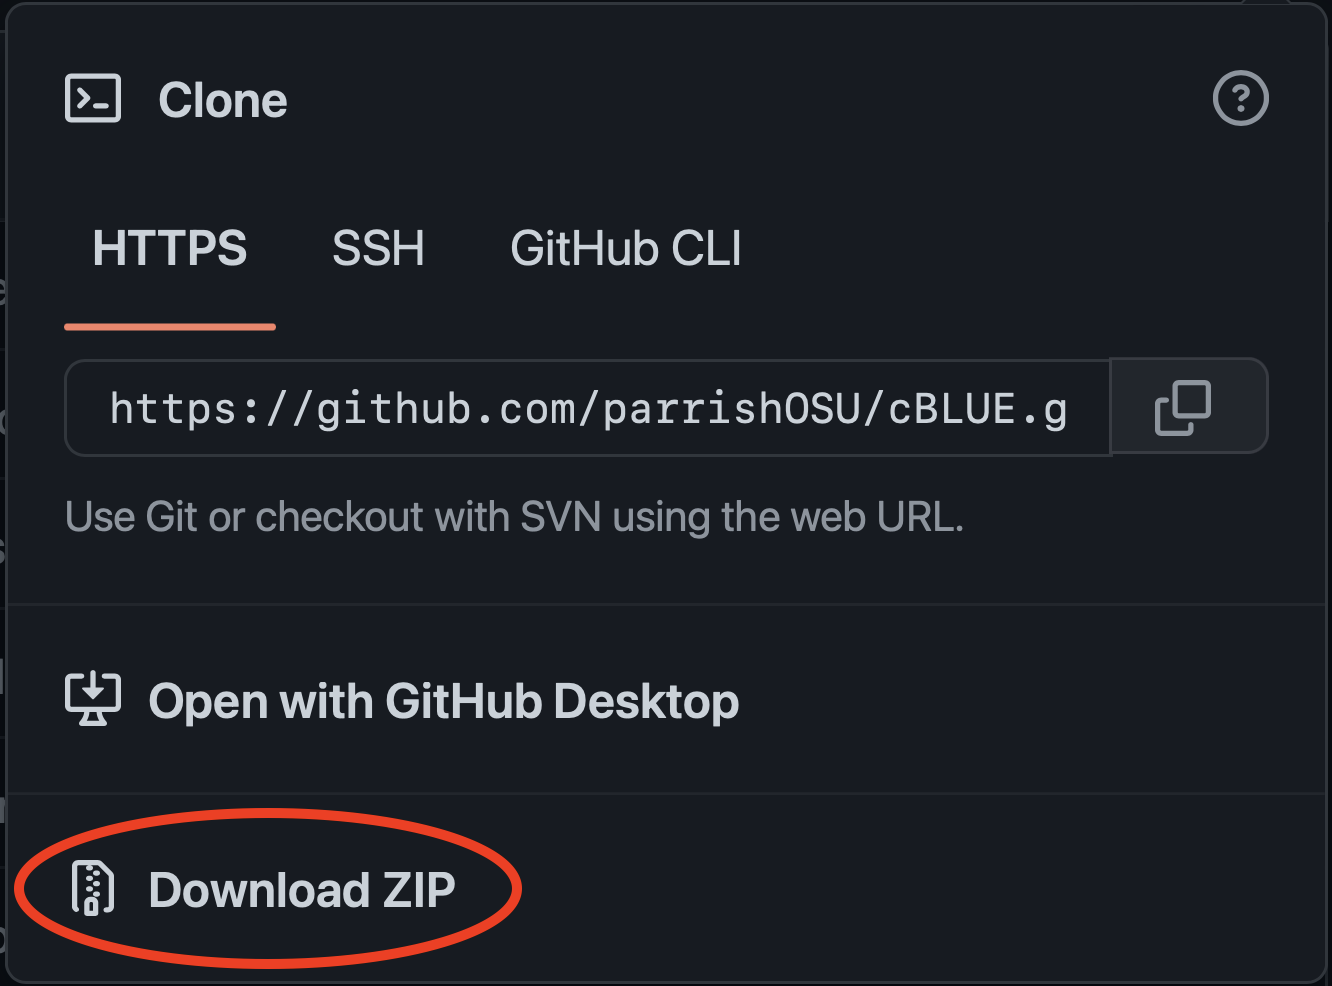
\includegraphics[height=5cm]{figs/cblue_download.png}
    \end{figure}
    \vspace{1em}
    \item Clone the repository using either your computer's terminal/command prompt or the Github Desktop Application:
    \paragraph{Terminal}
    \begin{enumerate}[label=(\alph*)]
        \item Navigate to the folder where you'd like to install cBLUE
        \colorbox{lightgray}{\begin{minipage}{\linewidth}
          \texttt{\$ cd location/of/cBLUE}
        \end{minipage}}
        \vspace{1em}
        \item Clone the repository using the url from github
        \colorbox{lightgray}{\begin{minipage}{\linewidth}
          \texttt{\$ git clone https://github.com/parrishOSU/cBLUE.github.io.git}
        \end{minipage}}
    \end{enumerate}
    \paragraph{GitHub Desktop}
    \begin{enumerate}[label=(\alph*)]
        \item Open GitHub Desktop and locate the "Add" button
        \begin{figure}[H]
            \centering
            
\includegraphics[height=1cm]{figs/add.png}
        \end{figure}
        \vspace{1em}
        \item Under "Add" choose "Clone Repository" and select "URL"
        \begin{figure}[H]
            \centering
            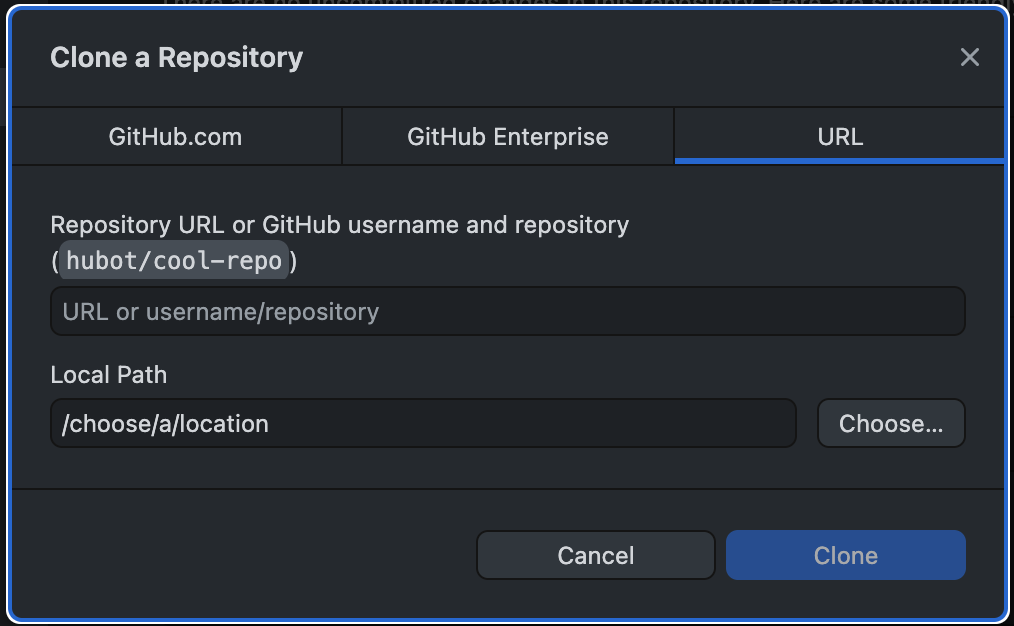
\includegraphics[height=5cm]{figs/GitHubDesktop.png}
        \end{figure}
        \vspace{1em}
        \item Enter the path to the location you'd like to install cBLUE and paste the url found in Step 2 in the appropriate boxes
        \vspace{1em}
        \item Press the "Clone" button to begin download
        \begin{figure}[H]
            \centering
            
\includegraphics[height=1cm]{figs/clone.png}
        \end{figure}
    \end{enumerate}
    \vspace{1em}
    \item Once the download is complete, check that the folder \texttt{cBLUE.github.io} is in the desired location.
\end{enumerate}
\subsubsection{Download as \texttt{.zip}}
\begin{enumerate}
    \item In a web browser, navigate to \url{https://github.com/parrishOSU/cBLUE.github.io}
    \vspace{1em}
    \item In the top right of the repository, locate the green \texttt{code} menu and click "Download Zip"
    \begin{figure}[H]
        \centering
        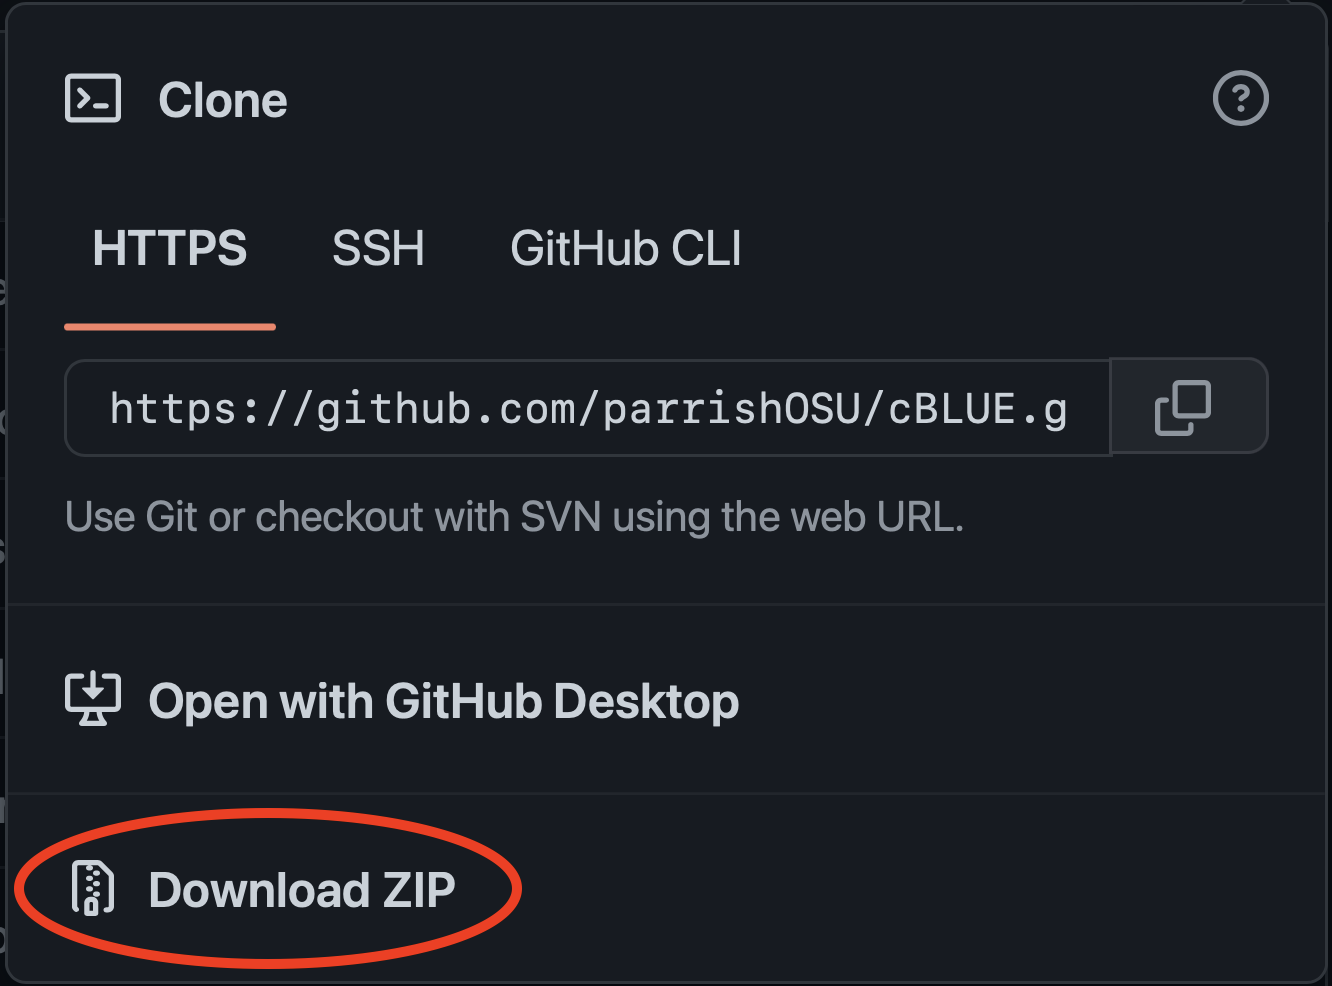
\includegraphics[height=5cm]{figs/cblue_download_zip.png}
    \end{figure}
    \vspace{1em}
    \item Once the download is complete, move the \texttt{.zip} to your desired location and extract to \texttt{cBLUE.github.io}.
\end{enumerate}

\subsection{Install cBLUE Dependencies}
cBLUE is designed to be a cross-platform software, therefore this installation guide should be valid for all Windows, MacOS, and Linux users. However, cBLUE does require Python 3 to be installed on the user's machine, as well as all the Python library dependencies needed to run cBLUE. Additionally, while it is possible to install cBLUE using any Python package manager, we strongly suggest using \texttt{conda}, which can be downloaded for free  \href{https://www.anaconda.com/products/distribution}{here}. In this installation guide we provide instructions to install and run cBLUE using both the Anaconda Navigator GUI as well as the \texttt{conda} CLI.

\subsubsection{conda}
\begin{enumerate}
    \item In your computer's terminal/command prompt, navigate to \texttt{cBLUE.github.io}
    \colorbox{lightgray}{\begin{minipage}{\linewidth}
          \texttt{\$ cd location/of/cBLUE/cBLUE.github.io}
    \end{minipage}}
    \vspace{1em}
    \item Locate the file \texttt{cblue.yml}
    \vspace{1em}
    \item Create a new virtual environment using the command
    \colorbox{lightgray}{\begin{minipage}{\linewidth}
          \texttt{\$ conda env create -f cblue.yml}
    \end{minipage}}
    \vspace{1em}
    \item cBLUE dependencies should begin downloading shortly.
    \vspace{1em}
    \item Once all dependencies have successfully downloaded, activate the new environment using the command
    \colorbox{lightgray}{\begin{minipage}{\linewidth}
        \texttt{\$ conda activate cblue}
    \end{minipage}}
    \vspace{1em}
    \item To check that the dependencies are installed properly, use the command
    \colorbox{lightgray}{\begin{minipage}{\linewidth}
        \texttt{\$ python CBlueApp.py}
    \end{minipage}}
\end{enumerate}

\subsubsection{Anaconda Navigator}
\begin{enumerate}
    \item Open "Anaconda Navigator" and navigate to the "Environments" menu on the left hand side.
    \vspace{1em}
    \item Locate the "Import" button on the bottom left
    \begin{figure}[H]
        \centering
        
\includegraphics[height=2cm]{figs/IMPORT.png}
    \end{figure}
    \vspace{1em}
    \item In the "Import New Environment" dialog box, enter "cblue" for "Name" and navigate to the file \texttt{cblue.yml} for the "Specification File"
    \begin{figure}[H]
        \centering
        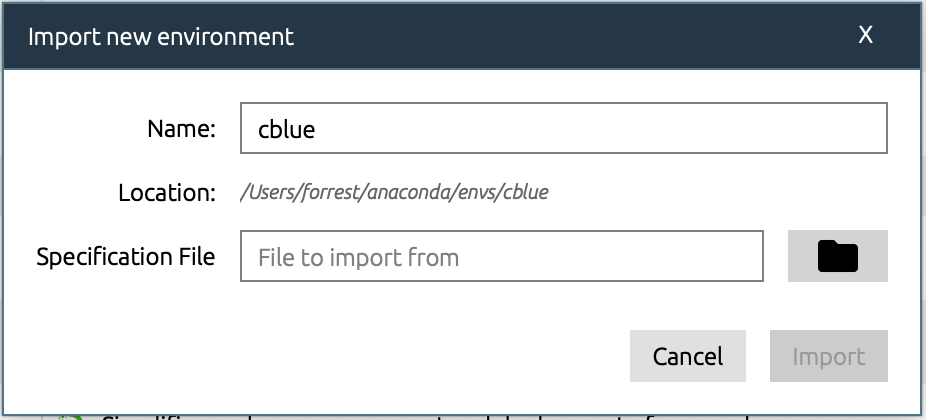
\includegraphics[height=3cm]{figs/import_window.png}
    \end{figure}
    \vspace{1em}
    \item Click "Import"
    \vspace{1em}
    \item Once the downloads are complete, locate "cblue" in the environments list and click on it to activate. A green triangle should appear next to the environment name once it is activated.
    \vspace{1em}
    \item To check that the dependencies are installed correctly, click the green triangle next "cblue" and select "Open Terminal"
    \begin{figure}[H]
        \centering
        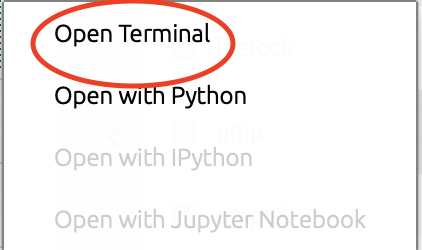
\includegraphics[height=3cm]{figs/open_term.png}
    \end{figure}
    \vspace{1em}
    \item Navigate to the location of \texttt{cBLUE.github.io}
    \colorbox{lightgray}{\begin{minipage}{\linewidth}
          \texttt{\$ cd location/of/cBLUE/cBLUE.github.io}
    \end{minipage}}
    \vspace{1em}
    \item Open cBLUE using the command
    \colorbox{lightgray}{\begin{minipage}{\linewidth}
        \texttt{\$ python CBlueApp.py}
    \end{minipage}}
\end{enumerate}

\section{User Guide}
This section provides step-by-step instructions to perform a Total Propagated Uncertainty (TPU) estimation from bathymetric lidar data. In order to perform this estimation, it is assumed that the user has properly install cBLUE and its dependencies. If cBLUE or its dependencies are not installed, please refer to Section 2 of this manual.

\vspace{1em}

In order to perform a TPU estimation using cBLUE, it is necessary to have two sets of files: at least one \texttt{.las} file containing information on the lidar return signal and at least one corresponding SBET (\texttt{.txt}) file containing information on the sensor trajectory at the time of each lidar pulse. These files are (usually) obtained directly from the sensor platform. Further information on these file types is outside the scope of this manual.

\vspace{1em}

To open cBLUE, in the terminal of your choosing, execute the following command from inside the \texttt{cBLUE.github.io} folder.
\colorbox{lightgray}{\begin{minipage}{\linewidth}
        \texttt{\$ python CBlueApp.py}
\end{minipage}}

\vspace{1em}

The following message should appear in your terminal:
\begin{figure}[H]
    \centering
    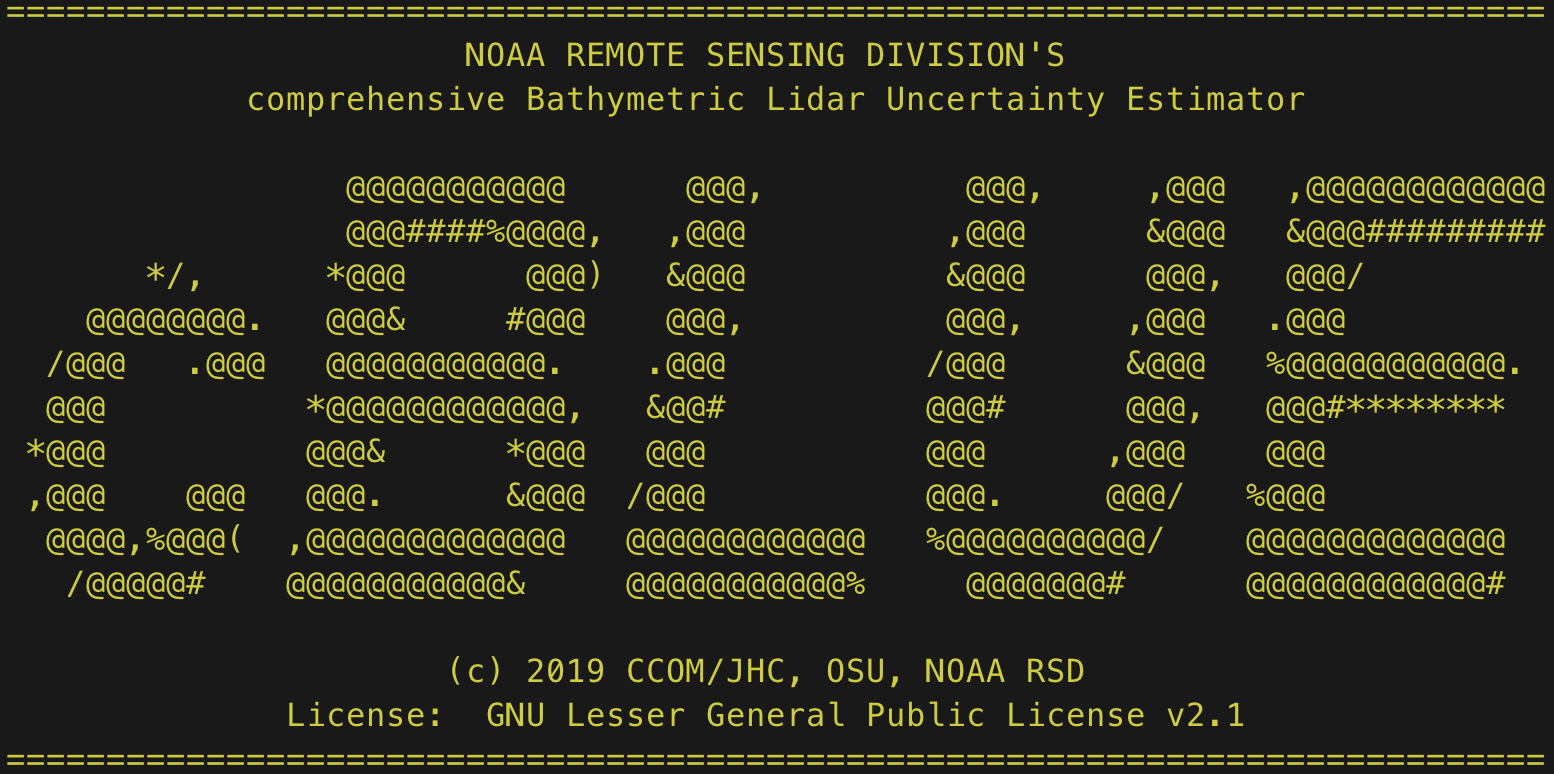
\includegraphics[height=4cm]{figs/cblue_term_logo.png}
\end{figure}

(Note: the \texttt{cblue} conda environmental must be installed and activated in order to run cBLUE. If cBLUE fails to open, it is likely that your dependencies are not installed or the environment is deactivated. Refer to Section 2 of this manual for information on resolving these issues.)



\subsection{Data Directories}
The first step in performing a TPU estimation using cBLUE is to point the software to the \texttt{.las} and SBET (\texttt{.txt}) files on your system. This is done using the Data Directories selection menus. 

\begin{figure}[H]
    \centering
    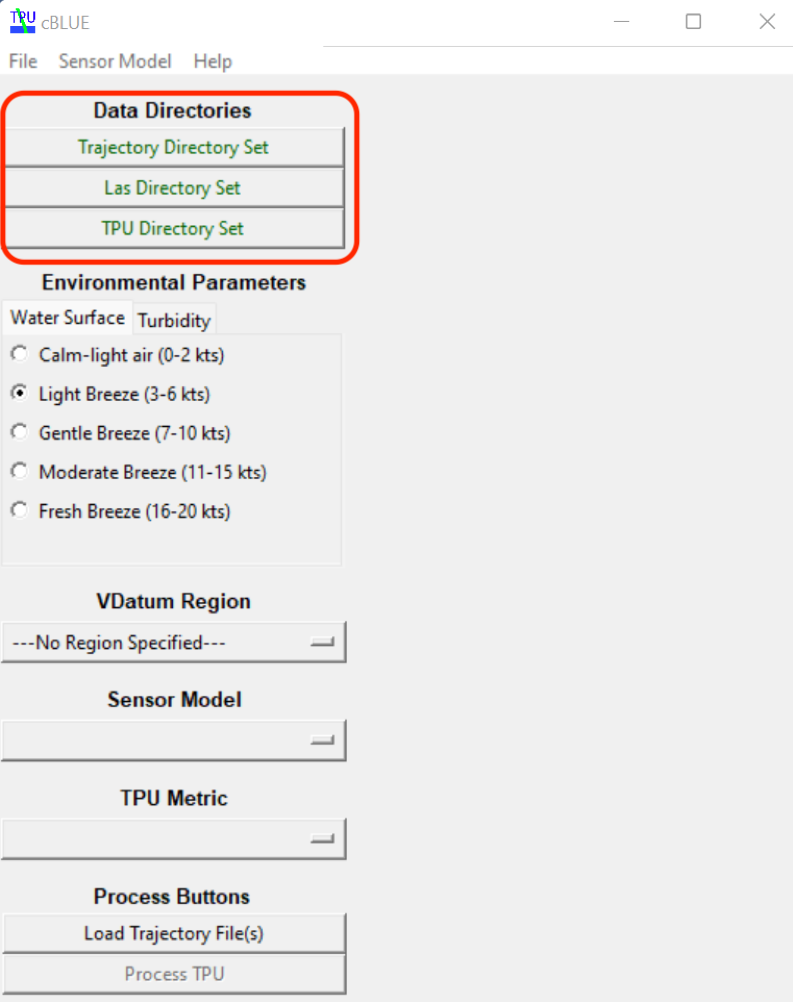
\includegraphics[height=7cm]{figs/cblue_menu_data_dir.png}
\end{figure}

\subsubsection{Trajectory}
The "Trajectory Directory Set" menu allows the user to select the location of the SBET files containing the sensor trajectory parameters at the time of each laser pulse.

\begin{figure}[H]
    \centering
    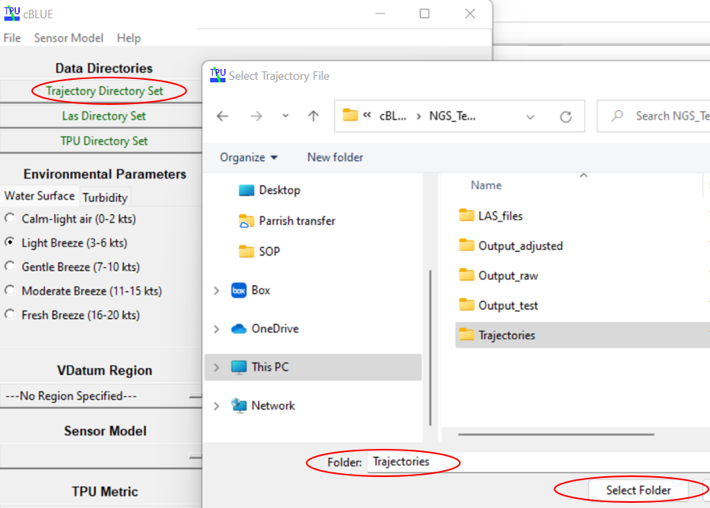
\includegraphics[height=6cm]{figs/select_traj.png}
\end{figure}

These files are usually generated by the lidar system and therefore their generation and file standards are outside the scope of this manual, however a brief overview of ASCII SBET formatting is avaible in \hyperref[appendix:SBET]{Appendix A}. If you run into issue regarding the SBET files, please consult the lidar system's user manual or contact the manufacturer before raising an issue with the cBLUE maintenance team, as these issues are often the result of erroneous data and are therefore difficult to reproduce/troubleshoot. An example of SBET files is shown in the figure below.

\begin{figure}[H]
    \centering
    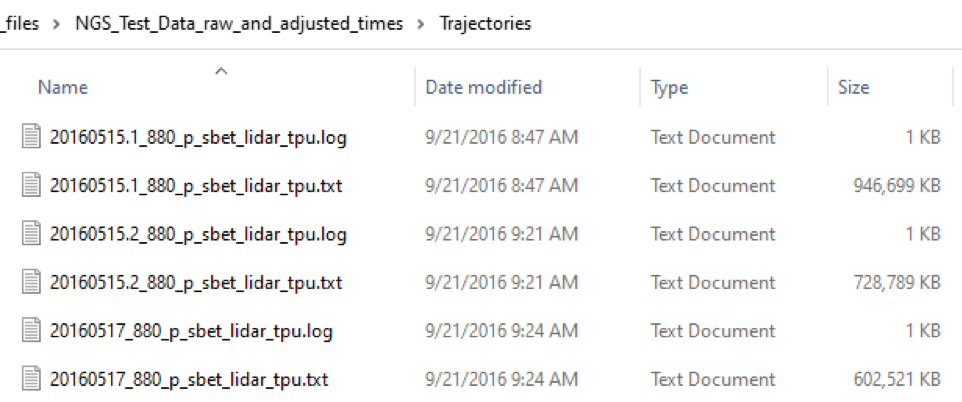
\includegraphics[width=10cm]{figs/example_data.png}
\end{figure}


\subsubsection{Las Files}
The "Las Directory Set" menu allows the user to select the location of the \texttt{.las} files containing the point cloud coordinates from each laser pulse. 

\begin{figure}[H]
    \centering
    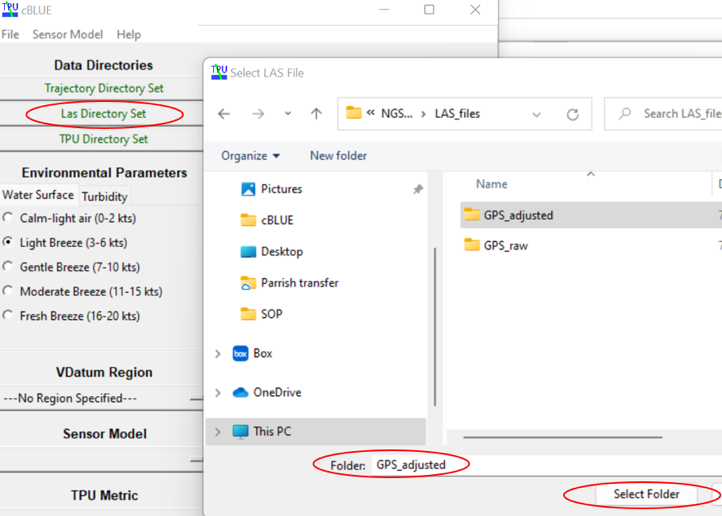
\includegraphics[height=6cm]{figs/select_las.png}
\end{figure}

Currently, given the popularity of \texttt{.las}, especially in the bathymetric lidar community, these are the only files types supported. There are no plans to add further file types\footnote{As of cBLUE V3.0, compressed LAS files (\texttt{.laz}) are also accepted by cBLUE.}. Additionally, note that the GPS times in the LAS file should be Adjusted Standard GPS Time. This is important because the GPS times are how cBLUE matches up points in the LAS file with corresponding records from the trajectory. For more information on LAS file specifications, please refer to the ASPRS LASER (LAS) FILE FORMAT EXCHANGE ACTIVITIES, found \href{https://www.asprs.org/divisions-committees/lidar-division/laser-las-file-format-exchange-activities}{here}.

\subsubsection{TPU Directory}
The "TPU Directory Set" menu allows the user to select the location of the output files. 

\begin{figure}[H]
    \centering
    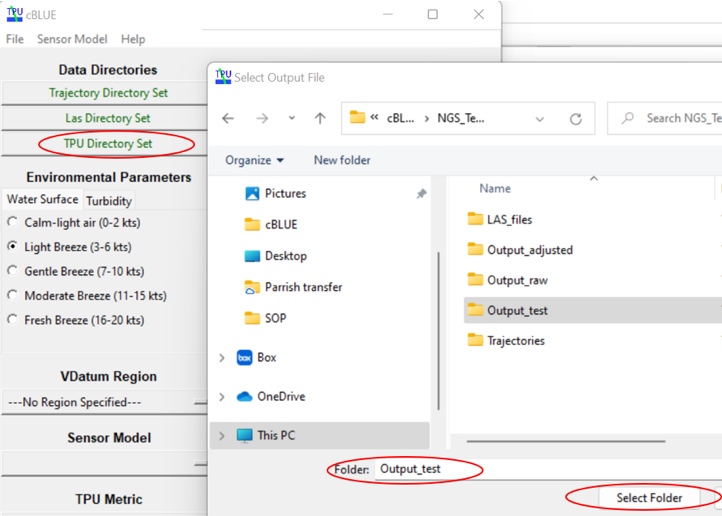
\includegraphics[height=6cm]{figs/select_out.png}
\end{figure}

The files output by cBLUE will match the \texttt{.las} files in the "Las Directory Set" location, with \texttt{\_TPU} appended to the file name. These output files will contain the TPU as ExtraBytes fields. More information on LAS ExtraBytes can be found \href{https://www.asprs.org/divisions-committees/lidar-division/laser-las-file-format-exchange-activities}{here}.

\subsection{Environmental Parameters}
cBLUE operates by using a combined subaerial and subaqeuous model. The subaqeuous model is designed to simulate the range of possible values for each laser shot, given a set of environmental parameters. Therefore, it is important that the user tune these parameters to reflect the best approximation of the water conditions at the time the bathymetric survey was conducted. 

\begin{figure}[H]
    \centering
    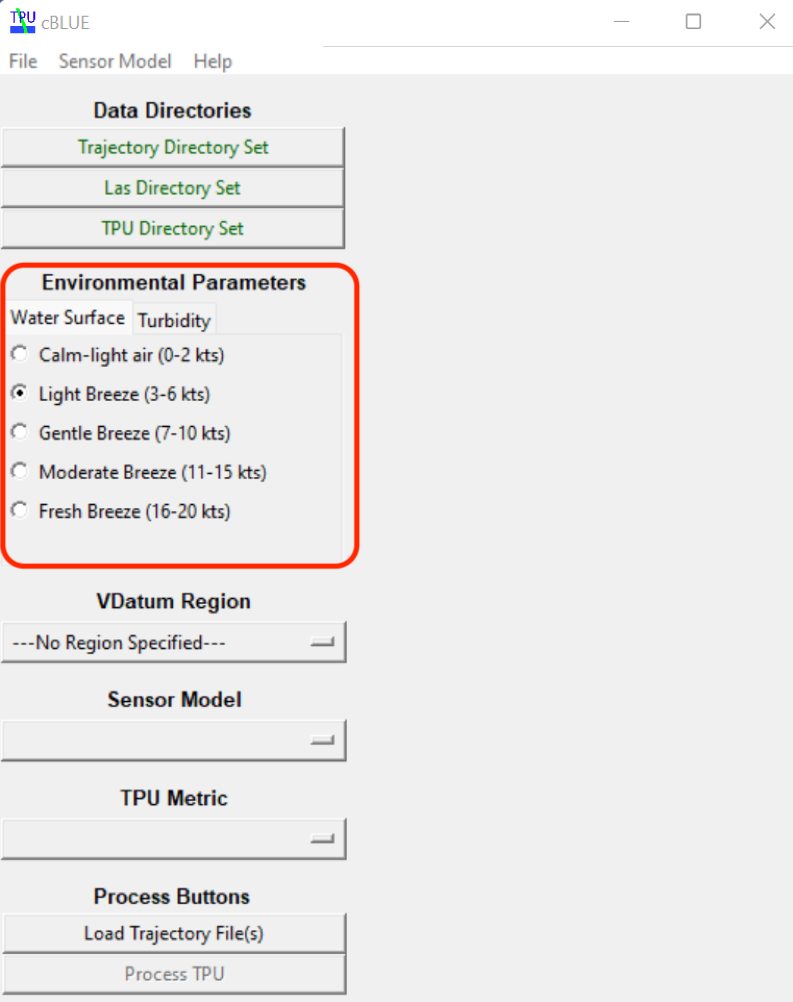
\includegraphics[height=7cm]{figs/cblue_menu_env_params.png}
\end{figure}

\subsubsection{Water Surface}
The "Water Surface" menu allows the user to select the range of water surface parameters that best approximate the water surface conditions at the time of the bathymetric survey.

\vspace{1em}

\textit{(Note: cBLUE V2.X included an option to model the water surface from using the pointcloud data. This option has been removed as of cBLUE V3.0. For more information on why this option was removed, please refer to Section 4 of this manual).}

\subsubsection{Turbidity}
The "Turbidity" menu allows the user to select the range of turbidity parameters that best approximate the water clarity conditions at the time of the bathymetric survey.

\begin{figure}[H]
    \centering
    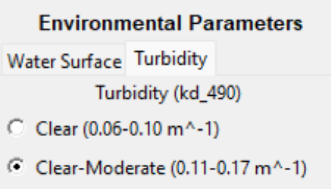
\includegraphics[width=7cm]{figs/env_params.png}
\end{figure}

\subsection{VDatum Region}
Vertical datum uncertainty is a component uncertainty often included in bathymetric TPU modeling. The "VDatum Region" menu allows the user to select a VDatum region to use in the modeling process. The purpose of this setting is to enable users to include VDatum datum transformation uncertainty (\url{https://vdatum.noaa.gov/docs/est_uncertainties.html}) as a component uncertainty in the TPU computation.  However, this parameter is not required to perform the uncertainty estimation and may be left as "--No Region Specified--" by the user.

\begin{figure}[H]
    \centering
    
\includegraphics[width=7cm]{figs/vdat.png}
\end{figure}

\subsection{Sensor Model}
As of cBLUE V3.0, there are 3 lidar sensor platforms available in cBLUE. These include the Riegl VQ-880-G, Leica Chiroptera 4X, and Leica Hawkeye 4X. The Parrish Group at OSU is also actively working to develop subaqeuous models for more sensors to be included in future versions of cBLUE. To request a sensor model, please post an issue on the cBLUE GitHub page \href{https://github.com/parrishOSU/cBLUE.github.io/issues}{here}.

\begin{figure}[H]
    \centering
    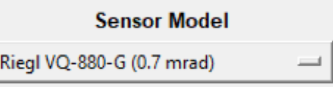
\includegraphics[width=7cm]{figs/sensor.png}
\end{figure}

\begin{figure}[H]
    \centering
    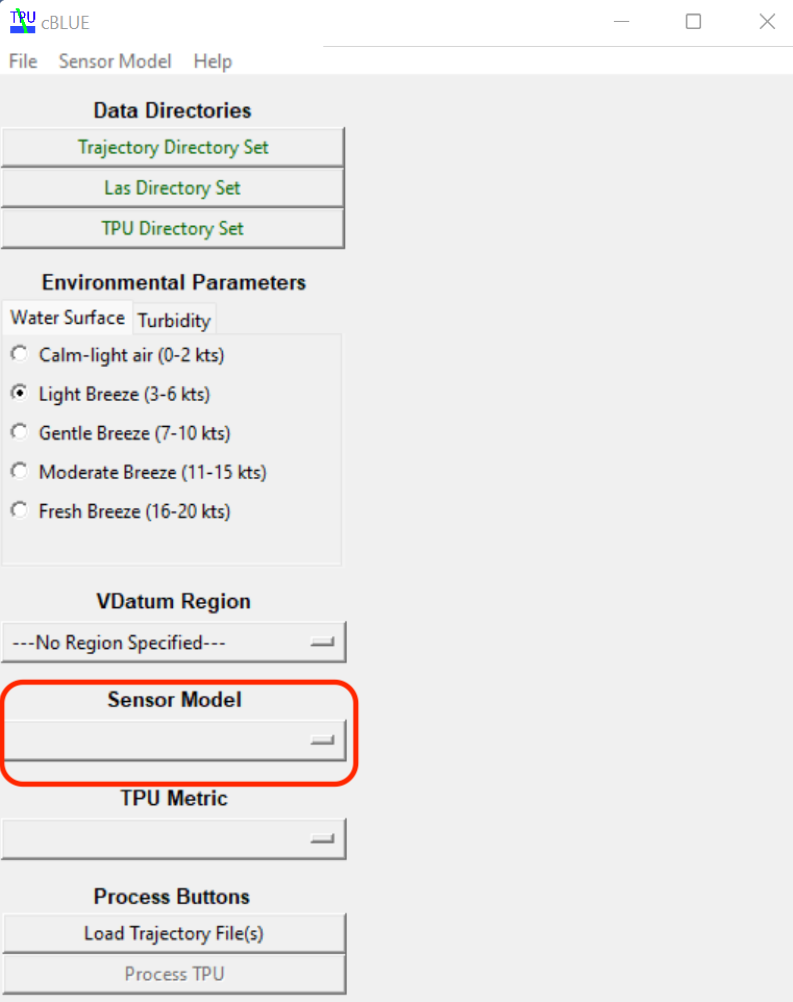
\includegraphics[width=7cm]{figs/cblue_menu_sensor.png}
\end{figure}

\subsubsection{Riegl VQ-880-G}
The Riegl VQ-880-G sensor includes a programmable beam with a selectable beam divergence. Subaqueous models are available for each beam divergence in cBLUE. The following values are the beam divergences modeled by cBLUE in milliradians.
\begin{itemize}
    \item 0.7 mrad
    \item 1.0 mrad
    \item 1.5 mrad
    \item 2.0 mrad
\end{itemize}
\subsubsection{Leica Chiroptera 4X}
As of V3.0, a subaqeuous model is available to estimate TPU from LAS data collected by Leica Chiroptera 4x sensors.

\subsubsection{Hawkeye 4X}
As of V3.0, a subaqeuous model is available to estimate TPU from LAS data collected by Leica Hawkeye 4x sensors. (Note: the "shallow" channel of the Hawkeye 4x sensor is identical to the Chiroptera 4x. Therefore, similarity between estimates calculated using either of these two models on the same dataset may be nearly identical in shallow waters.)

\subsection{TPU Metric}
As of cBLUE V3.0, users may select to output TPU values at either 95\% Confidence or 1-$\sigma$. 

\begin{figure}[H]
    \centering
    
\includegraphics[width=7cm]{figs/metric.png}
\end{figure}

Previous versions of cBLUE defaulted to 1-$\sigma$. Conversion between 1-$\sigma$ and 95\% Confidence for Total Vertical Uncertainty (TVU) and Total Horizontal Uncertainty (THU) can also be performed after estimation using the relationships below:
\paragraph{TVU:}
\begin{equation*}
    \text{95\% Confidence} = 1.96 \times (\text{1-$\sigma$})
\end{equation*}

\paragraph{THU:}
\begin{equation*}
    \text{95\% Confidence} = 1.7308 \times (\text{1-$\sigma$})
\end{equation*}

\subsection{Output Options}
cBLUE V3.0 allows the user to choose between exporting the estimated TVU/THU solely as ExtraBytes in the new LAS file, or to also include a comma separated values (CSV) table with the TVU/THU. This option may be suitable for users with small datasets who wish to work with the resulting uncertainties in software that does not handle LAS files, or those who are unfamiliar with the LAS format. However, the process of building and saving a CSV file with information for each point can be slow and is therefore not recommended for users with large files, or a large number of files. 

\vspace{1em}

The information included in the optional output CSV is detailed in Table \ref{tab:csv}. 
\begin{table}[H]
    \centering
    \begin{tabular}{c|l}
        \textbf{Field} & \textbf{Description} \\
        \hline \\
        GPS Time & The GPS Time of each point in the format \\
        \ & of the corresponding input LAS/LAZ file \\
        \hline \\
        X &  The X coordinate of each point in the format \\
        \ & of the corresponding input LAS/LAZ file\\
        \hline \\
        Y & The Y coordinate of each point in the format \\
        \ & of the corresponding input LAS/LAZ file \\
        \hline \\
        Z & The Z coordinate of each point in the format \\
        \ & of the corresponding input LAS/LAZ file \\
        \hline \\
        THU & The Total Horizontal Uncertainty of each point \\
        \ & as estimated by cBLUE \\
        \hline \\
        TVU & The Total Vertical Uncertainty of each point \\
        \ & as estimated by cBLUE \\
        \hline \\
        Classification & The classification of each point as specified \\
        \ & in the input LAS/LAS file \\
        \hline
    \end{tabular}
    \caption{Output CSV fields}
    \label{tab:csv}
\end{table}

While other fields can be added to the CSV by modifying cBLUE's code, it is strongly recommended that users wishing to access additional fields simply export as ExtraBytes and use the \texttt{las2txt} tool from LASTools, which can be downloaded \href{https://rapidlasso.com/las2txt/}{here}.

\subsection{Load Trajectory Files}
After indicating the appropriate data directories and selecting the appropriate parameters for the lidar survey, the user should press the "Load Trajectory Files" button to process the SBET data.

\begin{figure}[H]
    \centering
    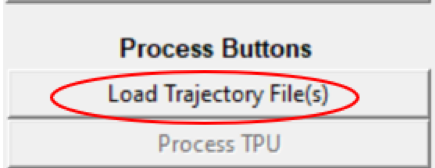
\includegraphics[width=7cm]{figs/loadtraj.png}
\end{figure}

The trajectories may take a few moments to load, during which time you can track the progress in your terminal/command window.

\begin{figure}[H]
    \centering
    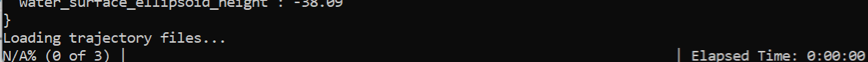
\includegraphics[width=15cm]{figs/term_loadtraj.png}
\end{figure}

\subsection{Process TPU}
Once the trajectory files are successfully loaded, the "Process TPU" button will become clickable. Clicking this button will initiate the TPU estimation model.

\subsubsection{Water Surface Ellipsoid Height}
The "Process TPU" will bring up a window asking the user to enter the ellipsoid height of the water surface. The purpose of this parameter is to enable a slant range correction. This value should be close, but it does not need to be perfect, as changes in this parameter generally only impact the computed TVU on the order of millimeters. The preferred method of obtaining this value is to use an average ellipsoid height of water surface (Class 41) points in the LAS file. Alternately, method of obtaining an approximate value for this parameter is to use \href{https://vdatum.noaa.gov/vdatumweb/}{VDatum online} to compute the separation between the NAD83 ellipsoid and one of the following tidal datums, depending on which was closest to the water level at the time the bathymetric lidar dataset was acquired: mean lower low water (MLLW), mean low water (MLW), mean tide level (MTL), mean high water (MHW), or mean higher high water (MHHW). If the stage of tide at the time the bathymetric lidar was acquired is unknown, it is usually reasonably safe to select local mean sea level (LMSL) as the “to” datum; typically, this will only impact the computed TPU values on the order of millimeters.

\begin{figure}[H]
    \centering
    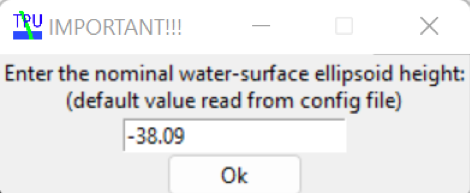
\includegraphics[width=7cm]{figs/nom_h20_surf.png}
\end{figure}

\subsubsection{Monitoring Progress}
After clicking "Ok" on the Water Surface Ellipsoid Height window, cBLUE will begin to estimate TPU. To monitor the progress of cBLUE, please refer to your terminal/command window. When the model has completed successfully, you will see the following:
\begin{figure}[H]
    \centering
    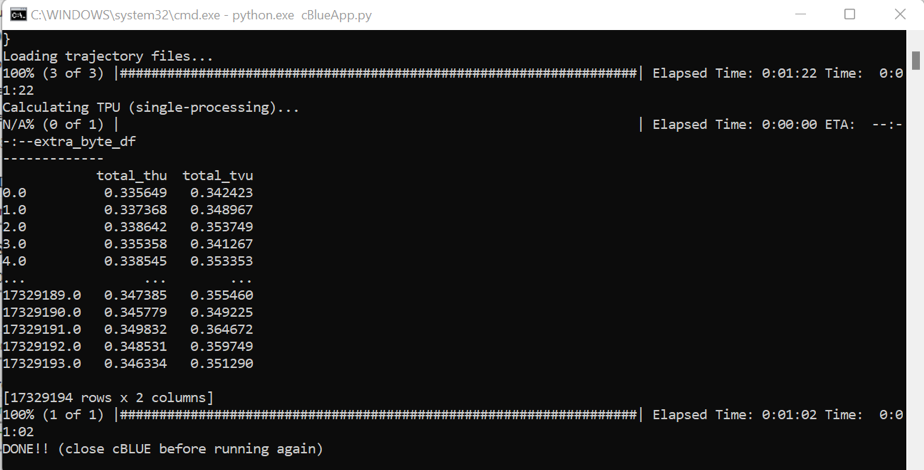
\includegraphics[width=15cm]{figs/terminal_output.png}
\end{figure}

\section{Updates -- V3.0}       
\label{sec:updates}    
\vspace{-.1cm}
The following list details the major updates associated with cBLUE V3.0. This is not a comprehensive list of updates to the code, which can be found under the github commit history associated with cBLUE.
\begin{itemize}
    \item Added Sensor Models:
    \begin{itemize}
        \item Riegl VQ 880-G :
        \begin{itemize}
            \item 0.7 mrad
            \item 1.0 mrad
            \item 1.5 mrad
            \item 2.0 mrad
        \end{itemize}
        \item Leica Chiroptera 4X
        \item Hawkeye 4X
    \end{itemize}
    \item Removed "Direct from Point Cloud" Option
    \item Added TPU Metric User Selection
    \item Updated Dependency (laspy 2.0 $\rightarrow$ laspy 3.0)
    \item Updated File Types (.laz files accepted)
    \item Added a "minimum" TPU value of 3.0 cm. Values below this threshold were determined to be erroneously small.
    \item Optional CSV output now available.
\end{itemize}

\section{Open Issues}       
\label{sec:issues}   
\vspace{-.1cm}
This section details the open "issues" for cBLUE. This is not a list of known bugs, but a list of possible additions and modifications that might be made to cBLUE. These additions may be tackled by members of the Parrish Group Cblue maintenance team at Oregon State University, or may be contributed by members of the cBLUE community pending review from the Parrish Group.

\begin{itemize}
    \item Additional Sensors
    \begin{itemize}
        \item Any additional sensor models generated by the cBLUE community are welcome and encouraged. If you've generated a subaqueous look up table using the Monte Carlo process detailed \href{link needed}{link needed}, we would be happy to help you implement it in cBLUE. 
    \end{itemize}
    \item \ 
\end{itemize}

\appendix
\section{ASCII SBET Format}
\label{appendix:SBET}
The format of the trajectory files needed for cBLUE is a custom ASCII SBET with the following format:
\begin{figure}[H]
    \centering
    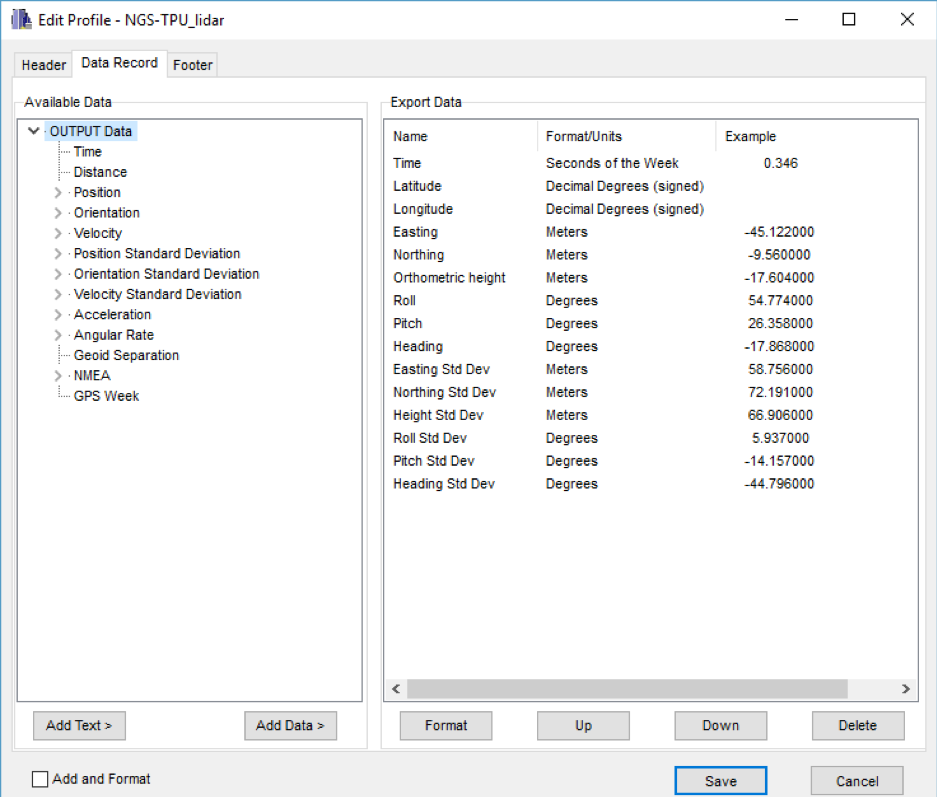
\includegraphics[width=15cm]{figs/SBET_format.png}
\end{figure}

\bibliographystyle{plain}
\nocite{*}
\bibliography{references.bib}
\end{document} 